\section{The SkelCL Programming Model}
\label{section:skelcl-programming-model}
\SkelCL (Skeleton Computing Language) is a high-level programming model targeting multi-\GPU system.
It is developed as an extension of the standard \OpenCL programming model~\cite{OpenCL}.
\SkelCL adds three main high-level features to \OpenCL which we identified as desirable in~\autoref{section:requirements}:

\begin{itemize}
  \item \emph{parallel container data types} for unified memory management between host and devices;
  \item \emph{recurring patterns of parallelism} (\aka \emph{algorithmic skeletons}) for easily expressing parallel computation patterns;
  \item \emph{data distribution} and \emph{redistribution} mechanisms for programming multi-device systems.
\end{itemize}

\noindent
\SkelCL inherits all properties of \OpenCL, including its portability across different heterogeneous parallel systems.
\SkelCL is designed to be fully compatible with \OpenCL: arbitrary parts of a \SkelCL code can be written or rewritten in \OpenCL, without influencing program's correctness.

In the rest of the section we discuss the design of the \SkelCL programming model in more detail.
The implementation as a \Cpp library will be discussed in the next section.

% ============================================================================ %
\subsection{Parallel Container Data Types}
\label{section:skelcl-programming-model:container}
\SkelCL offers the application developer two container classes -- vector and matrix -- which are transparently accessible by both, host and devices.
The \emph{vector} abstracts a one-dimensional contiguous memory area while the \emph{matrix} provides an interface to a two-dimensional memory area.
When a container is created on the host, memory is allocated on the devices automatically;
when a container on the host is deleted, the memory allocated on the devices is freed automatically.

The main advantage of the container data types in \SkelCL as compared with \OpenCL is that the necessary data transfers between the host and devices are performed automatically and implicitly.
Before performing a computation on container types, the \SkelCL system ensures that all input containers' data is available on all participating devices.
This may result in implicit data transfers from the host to device memory, which in \OpenCL would require explicit programming, as we saw in~\autoref{section:opencl-example}.
Similarly, before any data is accessed on the host, the implementation of \SkelCL implicitly ensures that this data on the host is up-to-date by performing necessary data transfers automatically.
Thus, the container classes shield the programmer from low-level operations like memory allocation (on the devices) and data transfers between host and device.

Developing applications on two-dimensional data for modern parallel architectures is cumbersome and challenging, since efficient memory handling is essential for achieving good performance.
In case of \GPUs, exploiting the memory hierarchy by using the fast but small on-chip memory is key for high performance.
Therefore, in addition to the vector as a one-dimensional abstract data structure, \SkelCL offers a specific abstract data type for handling two-dimensional data, the matrix.

% The implementations of the algorithmic skeletons included in \SkelCL differentiate for their input container between vector and matrix, thus, offering optimized implementations for each case.


\subsection{Algorithmic Skeletons}
\label{section:skelcl-programming-model:skeletons}
In original \OpenCL, computations are expressed as compute \emph{kernels} which are executed in a parallel manner on an \OpenCL device:
as seen earlier the application developer must explicitly specify the parallelism by indicating how many instances of a kernel (called \emph{work items}) should be launched in parallel.
Communication between work items have to be implemented carefully to avoid race conditions and deadlocks.
In addition, kernels take pointers to device memory as input and contain program code for reading/writing single data items from/to it.
These pointers have to be used carefully, because no boundary checks are performed by \OpenCL.

To shield the application developer from these low-level programming issues, \SkelCL extends \OpenCL by introducing high-level programming patterns, called \emph{algorithmic skeletons}~\cite{Cole1991}.
Formally, a skeleton is a higher-order function that executes one or more user-defined (so-called \emph{customizing}) functions in a pre-defined parallel manner, thus hiding the details of parallelism and communication from the user~\cite{GorlatchCo2011}.

\SkelCL provides four basic data-parallel skeletons: \map, \zip, \reduce, and \scan;
as well as three more specialized skeletons: \mapOverlap, \stencil, and \allpairs.
In this section we will look at the basic skeletons, the specialized skeletons will be discussed in~\autoref{section:skelcl-programming-model:specialSkeletons}.
The four basic skeletons have been selected, because they have been proven to be useful for a broad range of applications.
Moreover, these skeletons can be efficiently implemented on \GPUs as their computation patterns match the data-parallel \SIMD (Singe Instruction, Multiple Data) execution model used by \GPUs.


\paragraph{The \map skeleton}
The \map skeleton is a well known basic algorithmic skeleton, applying the customizing function to each element of a container.
This skeleton originates from the functional world, where the \code{map} function is recognized as an important primitive for writing high-level code.
In many programming languages an equivalent sequential function exists, either known by the same name, like in Haskell or Python, or by other names, like \code{transform} in \Cpp, or \code{Select} in \Csharp.

In \SkelCL the \map skeleton can operate on vectors as well as matrices.
We start by formally define the skeleton on vectors:
\begin{definition}
  \label{definition:map}
  Let $\vec{x}$ be a vector of size $n$ with elements $x_i$ where $0 < i \leq n$.
  Let $f$ be a unary customizing function.
  The algorithmic skeleton \map is defined as follows:
  \begin{equation}
    map \big(\ f,\ [x_1, x_2, \dots, x_n]\ \big) = [f(x_1), f(x_2), \dots, f(x_n)]
  \end{equation}
\end{definition}
\noindent
The definition for matrices is similar:
\begin{definition}
  \label{definition:map:matrix}
  Let $M$ be an $n\times m$ matrix with elements $M_{i,j}$ where $0 < i \leq n$ and $0 < j \leq m$.
  Let $f$ be a unary customizing function.
  The algorithmic skeleton \map is defined as follows:
  \begin{equation}
    map\big(\ f,\ \DottedMatrix{M_{0,0}}{M_{0,m}}{M_{n,0}}{M_{n,m}} \big)
      = \DottedMatrix{f(M_{0,0})}{f(M_{0,m})}{f(M_{n,0})}{f(M_{n,m})}
  \end{equation}
\end{definition}
\noindent
The output container, either vector or matrix, can be computed in parallel, because the computation of each single element is independent of each other.

A simple possible application of the \map skeleton is negating all the values in a vector:
\begin{align*}
  neg(\vec{x}) &= map(\ -, \vec{x}\ )
\end{align*}


\paragraph{The \zip skeleton}
The \zip skeleton operates on two containers and combines them into one.
As the \map skeleton it is defined for vectors and matrices as well.
\begin{definition}
  \label{definition:zip}
  Let $\vec{x}$ and $\vec{y}$ be vectors of size $n$ with elements $x_i$ and $y_i$ where $0 < i \leq n$.
  Let $\oplus$ be a binary customizing operator.
  The algorithmic skeleton \zip is defined as follows:
  \begin{equation}
    \begin{split}
    zip \big(\ \oplus,\ [x_1, x_2, \dots, x_n],\ [y_1, y_2, \dots, y_n]\ \big)\\
      = [x_1 \oplus y_1, x_2 \oplus y_2, \dots, x_n \oplus y_n]
    \end{split}
  \end{equation}
\end{definition}
\noindent
Again the definition for matrices is similar:
\begin{definition}
  \label{definition:zip:matrix}
  Let $A$ and $B$ be $n\times m$ matrices with elements $A_{i,j}$ and $B_{i,j}$ where $0 < i \leq n$ and $0 < j \leq m$.
  Let $\oplus$ be a binary customizing operator.
  The algorithmic skeleton \zip is defined as follows:
  \begin{equation}
    \begin{split}
    zip\big( f,\ {\DottedMatrix{A_{0,0}}{A_{0,m}}{A_{n,0}}{A_{n,m}}},\
                 {\DottedMatrix{B_{0,0}}{B_{0,m}}{B_{n,0}}{B_{n,m}}}\big) \\
      = \DottedMatrix{A_{0,0} \oplus B_{0,0}}{A_{0,m} \oplus B_{0,m}}{A_{n,0} \oplus B_{n,0}}{A_{n,m} \oplus B_{n,m}}
    \end{split}
  \end{equation}
\end{definition}
\noindent
This definitions require the two input containers to be of exactly the same size.
The \zip skeleton is parallelizeable in the same manner as \map, as each element of the output container can be computed in parallel.

A possible application of the \zip skeleton is adding two vectors:
\begin{align*}
  add(\vec{x},\ \vec{y}) = zip(\ +, \vec{x},\ \vec{y}\ )
\end{align*}


\paragraph{The \reduce skeleton}
The \reduce skeleton computes a single value from a vector by successively applying the customizing function.
In \SkelCL the \reduce skeleton is only defined on vectors:
\begin{definition}
  \label{definition:reduce}
  Let $\vec{x}$ be a vector of size $n$ with elements $x_i$ where $0 < i \leq n$.
  Let $\oplus$ be an associative and commutative, binary customizing operator with the corresponding identity element $id$.
  The algorithmic skeleton \reduce is defined as follows:
  \begin{equation}
    reduce \big(\ \oplus,\ [x_1, x_2, \dots, x_n],\ id\ \big)
      = x_1 \oplus x_2 \oplus \dots \oplus x_n
  \end{equation}
\end{definition}
\noindent
Requiring the operator to be associative and commutative enables efficient parallel implementations.
The identity element $id$ can be used by the implementation, \eg, to initialize intermediate buffers. % TODO: think harder

A possible application of the \reduce skeleton is to find the maximum value of a vector:
\begin{align*}
  sumUp(\vec{x}) &= reduce(\ max, \vec{x},\ 0\ )\\
  \text{where: } max(a, b) &=
    \left\{
      \begin{array}{l l}
      a & \text{if } a \geq b\\
      b & \text{if } a < b
      \end{array}
    \right.
\end{align*}


\paragraph{The \scan skeleton}
The \scan skeleton (\aka prefix-sum) yields an output vector with each element obtained by applying the customizing function to the elements of the input vector up to the current element's index.
In \SkelCL the \scan skeleton is only defined on vectors:
\begin{definition}
  \label{definition:scan}
  Let $\vec{x}$ be a vector of size $n$ with elements $x_i$ where $0 < i \leq n$.
  Let $\oplus$ be an associative binary customizing operator with the corresponding identity element $id$.
  The algorithmic skeleton \scan is defined as follows:
  \begin{equation}
    \begin{split}
    scan \big(\ \oplus,\ [x_1, x_2, \dots, x_n],\ id\ \big) \\
      = [id, x_1 \oplus x_2,\ \dots,x_1 \oplus x_2 \oplus \cdots \oplus x_n]
    \end{split}
  \end{equation}
\end{definition}
\noindent
Even though, the \scan pattern seems inherently sequential, because each individual results contains the results of its predecessor, efficient parallel implementations does exist for this problem.
Blelloch~\cite{Blelloch1991} studies this parallel pattern in great details and efficient implementations for \GPUs exists~\cite{HarrisSeOw2007} following his algorithmic ideas.


\paragraph{Parallel Programming with Algorithmic Skeletons}
In \SkelCL, rather than writing low-level kernels, the application developer customizes suitable skeletons by providing application-specific functions which are often much simpler than kernels as they specify an operation on basic data items rather than containers.
Skeletons can be executed on both single- and multi-device systems.
In case of a multi-device system, the calculation specified by a skeleton is performed automatically on all devices available in the system.

Skeletons can be customized and composed to express more complex algorithms.
To demonstrate how to express computations with algorithmic skeletons let us consider three linear algebra applications:
scaling a vector with a constant, computing the sum of absolute values of a vector, and computing the dot product (\aka inner product) of two vectors.
These three applications are all part of the well known \emph{Basic Linear Algebra Subprograms (\BLAS)}~\cite{Dongarra2002,Dongarra2002a}.

For scaling a vector with a constant $\alpha$ we use the \map skeleton:
\begin{align*}
  scal(\vec{x}) &= map(\ f_{\alpha}, \vec{x}\ )\\
  \text{where: } f_{\alpha}(x_i) &= \alpha \cdot x_i
\end{align*}

\noindent
For computing the sum of absolute values we compose a \map and \reduce skeleton.
We use the $\circ$ to denote the sequential composition of two functions, \ie\ $f \circ g(x) = f(g(x))$.
\begin{align*}
  asum(\vec{x}) &= reduce(\ +\ ) \circ map(\ abs, \vec{x}\ )\\
  \text{where: } abs(a) &=
    \left\{
      \begin{array}{r l}
      a & \text{if } a \geq 0\\
      -a & \text{if } a < 0
      \end{array}
    \right.
\end{align*}

\noindent
To compute the dot product of two vectors we compose a \zip skeleton customized with multiplication and a \reduce skeleton customized with addition:
\begin{align*}
  dot(\vec{x}, \vec{y}) &= reduce(\ +\ ) \circ zip(\ *, \vec{x}, \vec{y}\ )
\end{align*}

\noindent
Algorithmic skeletons are not just limited to linear algebra applications, but can be used to implement a boarded range of application types as we will discuss in \autoref{chapter:skelcl-evaluation}.
Among others, we will see an implementation using algorithmic skeletons of the real-world medial imaging application example discussed at the beginning of this chapter.


% ============================================================================ %
\subsection{Data distribution and redistribution}
\label{section:skelcl-programming-model:distribution}

For multi-device systems, \SkelCL's parallel container data types (vector and matrix) abstract from the separate memory areas on multiple \OpenCL devices, \ie, container's data is accessible by each device.
Each device may access different parts of a container or may even not access it at all.
For example, when implementing work-sharing on multiple \GPUs, the \GPUs will access disjoint parts of input data, such that copying only a part of the vector to a \GPU would be more efficient than copying the whole data to each \GPU.

To simplify the partitioning of a container on multiple devices, \SkelCL supports the concept of \emph{distribution}.
A distribution describes how the container's data is distributed among the available devices.
It allows the application developer to abstract from the challenges of managing memory ranges which are shared or partitioned across multiple devices: the programmer can think of a distributed container as of a self-contained entity.



\begin{figure}[tb]
  \centering
  \begin{subfigure}{.3\textwidth}
    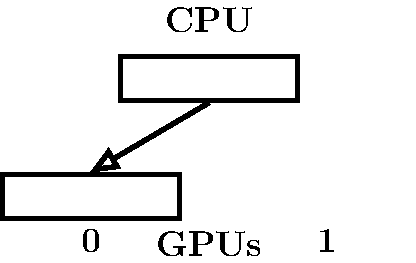
\includegraphics[width=\textwidth]{PaCT/singleDistribution_vector}
    \caption{\emph{single}}
    \label{fig:distributions:single}
  \end{subfigure}
  \hfill
  \begin{subfigure}{.3\textwidth}
    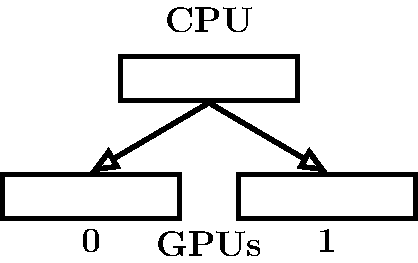
\includegraphics[width=\textwidth]{PaCT/copyDistribution_vector}
    \caption{\emph{copy}}
    \label{fig:distributions:copy}
  \end{subfigure}
  \hfill
  \begin{subfigure}{.3\textwidth}
    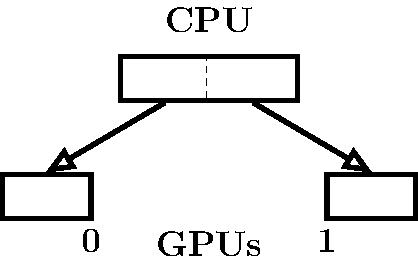
\includegraphics[width=\textwidth]{PaCT/blockDistribution_vector}
    \caption{\emph{block}}
    \label{fig:distributions:block}
  \end{subfigure}
  % \hfill
  % \begin{subfigure}{.22\textwidth}
  %   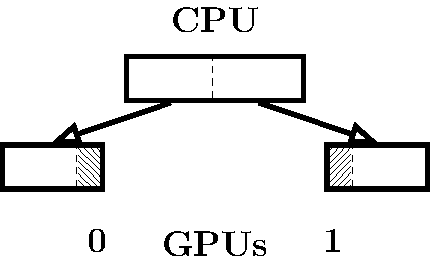
\includegraphics[width=\textwidth]{PaCT/overlapDistribution_vector}
  %   \caption{\emph{overlap}}
  %   \label{fig:distributions:overlap}
  % \end{subfigure}
  \caption{Distributions of a vector in SkelCL.}
  \label{fig:distributions}
  \bigskip
\end{figure}

\begin{figure}[tbp]
  \centering
  \begin{subfigure}{.22\textwidth}
    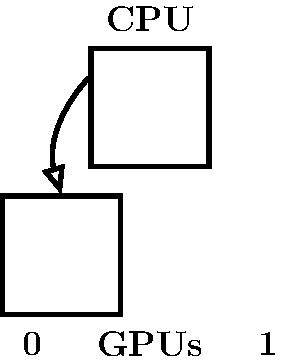
\includegraphics[width=\textwidth]{PaCT/singleDistribution_matrix}
    \caption{\emph{single}}
    \label{fig:distributions_matrix:single}
  \end{subfigure}
  \hfill
  \begin{subfigure}{.22\textwidth}
    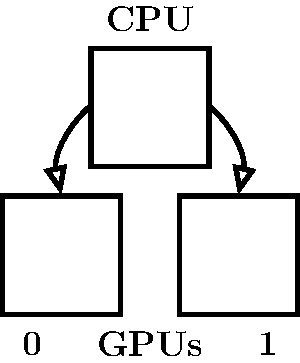
\includegraphics[width=\textwidth]{PaCT/copyDistribution_matrix}
    \caption{\emph{copy}}
    \label{fig:distributions_matrix:copy}
  \end{subfigure}
  \hfill
  \begin{subfigure}{.22\textwidth}
    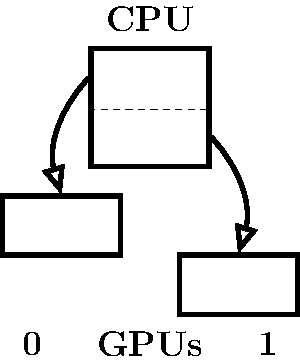
\includegraphics[width=\textwidth]{PaCT/blockDistribution_matrix}
    \caption{\emph{block}}
    \label{fig:distributions_matrix:block}
  \end{subfigure}
  % \hfill
  % \begin{subfigure}{.22\textwidth}
  %   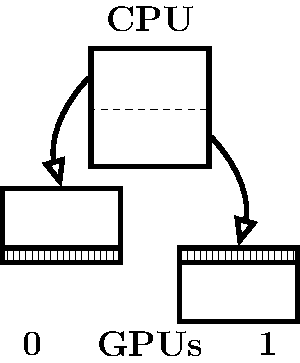
\includegraphics[width=\textwidth]{PaCT/overlapDistribution_matrix}
  %   \caption{\emph{overlap}}
  %   \label{fig:Distribution_matrixs:overlap}
  % \end{subfigure}
  \caption{Distributions of a matrix in SkelCL.}
  \label{fig:distributions_matrix}
\end{figure}


Three kinds of basic distributions are currently available in \SkelCL:
\emph{single}, \emph{copy}, and \emph{block} (see Figure~\ref{fig:distributions} for distributing a vector on a system with two \GPUs).
If distribution is set to \emph{single} (Figure~\ref{fig:distributions:single}), than vector's whole data is stored on a single \GPU (the first \GPU if not specified otherwise).
The \emph{copy} distribution (Figure~\ref{fig:distributions:copy}) copies vector's entire data to each available \GPU.
With the \emph{block} distribution (Figure~\ref{fig:distributions:block}), each \GPU stores a contiguous, disjoint chunk of the vector.

The same four distributions are provided also for the matrix data type as shown in Figure~\ref{fig:distributions_matrix}.
The \emph{block} distribution (Figure~\ref{fig:distributions_matrix:block}) splits the matrix into chunks of rows, which simplifies the implementation.

% TODO: move to block
% In particular the overlap distribution splits the matrix into one chunk for each GPU; in addition, each chunk contains a number of continuous rows from the neighboring chunks.
% A parameter -- the \emph{overlap size} -- specifies the number of rows at the borders of a chunk which are copied to the two neighboring GPUs.
% Figure~\ref{fig:Distribution_matrix:overlap} illustrates the overlap distribution:
% GPU 0 receives the top chunk ranging from the top row to the middle, while GPU 1 receives the second chunk ranging from the middle row to the bottom.
% The marked parts are called \emph{overlap region} they are the same on both GPUs.

The application developer can set the distribution of containers explicitly, otherwise every skeleton selects a default distribution for its input and output containers.
Container's distribution can be changed at runtime:
this implies data exchanges between multiple \GPUs and the \CPU, which are performed by the \SkelCL implementation implicitly.
As seen earlier in this chapter (Listing~\ref{lst:lmosem:redistribution}) implementing such data transfers in the standard \OpenCL is a cumbersome task:
data has to be downloaded to the \CPU before it is uploaded to the \GPUs, including the corresponding length and offset calculations;
this results in a lot of low-level code which becomes completely hidden when using \SkelCL.

A special situation arises when the distribution is changed from the \emph{copy} distribution to any other distribution.
In this case each \GPU holds its own full copy of the data which might have been modified locally on each \GPU.
In order to maintain \SkelCL's concept of a self-contained container, these different versions are combined using a user-specified function when the distribution is changed.
If no function is specified, the copy of the first \GPU is taken as the new version of the container; the copies of the other \GPUs are discarded.


% ============================================================================ %
\subsection{More Complex Algorithmic Skeletons}
\label{section:skelcl-programming-model:specialSkeletons}

The basic algorithmic skeletons presented in~\autoref{section:skelcl-programming-model:skeletons} are long known in the functional and algorithmic skeleton community.
In this section we will introduce three new algorithmic skeletons, which are more specialized and, thus, more restrictive.
By limiting the use cases of these novel algorithmic skeleton we are able to make more assumptions of the parallelization and provide optimized implementations on modern multi-\GPU systems.

Two of these new skeletons -- \mapOverlap and \stencil -- are targeted towards \emph{stencil} (\aka nearest neighbor) computations, which are computations performed for every element of a container while including neighboring elements in the computation.
The third new skeleton (\allpairs) allows to combine two matrix containers in an all-to-all fashion, which is a pattern used in application like n-body simulations or matrix matrix multiplication.

For each skeleton we will first formally define it before looking at possible use cases.
The implementations targeting multi-\GPU systems will be described in~\autoref{section:skelcl-library}.


\paragraph{The \mapOverlap Skeleton}


\paragraph{The \stencil Skeleton}


\paragraph{The \allpairs Skeleton}













































